%title:
%improving 2DoF pixel-based image synthesis of 360deg viewpoints using flow-based interpolation
%2DoF pixel-based synthesis of 360deg viewpoints using flow-based interpolation
%2 degree of freedom pixel-based synthesis of 360deg viewpoints with flow-based interpolation
%pixel-based synthesis of 360\degree viewpoints using flow-based interpolation
\chapter{Introduction}

Over the past decade, Virtual Reality (VR) technology has experienced a resurgence in popularity due to the development of a number of affordable, consumer-quality head-mounted displays\footnote{The price of a consumer-quality VR headset is between approximately 20 and 1000 USD as of January 2021, including headsets for use with a smartphone (\url{https://www.tomsguide.com/us/best-vr-headsets,review-3550.html}, \emph{accessed Jan 13, 2021})}. These displays allow a user to experience and interact with a virtual environment in 3D, for example by playing games, or by taking virtual tours of cities, historical landmarks, or remote locations in nature\footnote{``10 of the best virtual reality travel experiences'', Paul Joseph, Travelmag (\url{https://www.travelmag.com/articles/virtual-reality-travel-experiences/}, \emph{accessed Jan 13, 2021})}.

Some of these environments are modeled meticulously in 3D, while others use 360\degree images taken at the locations. Often, the modeled environments allow a lot of freedom of movement, enabling the user to ``walk'' around and inspect elements of the scene at will. Unfortunately, modeling a real environment by hand to be viewed interactively requires an enormous amount of effort and even then it is very unlikely to achieve photo-realism. The alternative is to capture the location with a 360\degree camera, which records the entire surroundings in a single image. Viewing these images offers photo-realism (as they are actual photos), but often awkward navigation, for example forcing the user to jump from image to image, instead of being able to ``walk'' smoothly around the scene. Nonetheless, the ease of capturing 360\degree images with modern 360\degree cameras, along with their significant advantage of photo-realism, makes this an attractive method for creating immersive VR environments.

The difficulties of navigating an environment captured by way of 360\degree cameras are not a new phenomenon. Virtual tours also exist outside of the realm of VR, viewed on regular computer or smartphone screens, for example interactive tours of museums, real-estate, or other locations of interest. A prominent example is Google's Street View, which allows users to navigate streets and monuments around the world by way of 360\degree images.

Whether a scene is viewed stereoscopically with a head-mounted display, or monoscopically on a flat screen, the greatest obstacle at the moment is the problem of interactive, user-driven navigation. Ideally, a user would be able to go anywhere they liked in the scene, and view anything they wanted from any angle and at any level of detail. Unfortunately, for environments captured by way of a 360\degree camera, this type of interaction would require a prohibitive amount of data, as well as being impossible to manually execute, since a separate image would have to be captured at every possible viewing position.

An alternative to capturing all of these viewpoints manually is to generate them digitally. This would require capturing much smaller subset of images and using these to generate uncaptured viewpoints. Generating new images based on already captured images is generally known as \emph{image-based rendering} (IBR), or image-based synthesis. There are many different approaches to synthesizing new images from captured ones, and they can generally be categorized by the degrees of freedom (DoF) that the technique can synthesize images with, as well as the type and amount of information extracted from the captured images.

The degrees of freedom that are necessary usually depend on the goal and requirements of the application: A virtual tour on a pre-defined path for example, would only require generating intermediate views between existing viewpoints (i.e. synthesis with 1DoF) for a smooth transition. For a less constrained virtual tour that enables the user to navigate freely, generating viewpoints with 2DoF at eye-height could be sufficient. The user could move around and look in any direction but not change their viewing height. Some applications may require three degrees of freedom, for example in order to enable the user to closely inspect certain objects from all angles.

Depending on the type of scene, the required fidelity, and real-time requirements, different IBR techniques leverage different amounts and types of information extracted from the input images. On one end of the scale, there are approaches that extract as much geometry information as possible from the set of images and try to reconstruct the 3D geometry of the image as closely as possible. These approaches suffer from the problem of extracting accurate geometry information, since errors in geometry can lead to unappealing results.
Then, there are approaches that try to extract some information from the image, such as feature correspondences, or motion vectors (optical flow), which enables interpolation between pairs of images, i.e. a smooth transition with 1DoF.
Approaches at the other end of the scale use no semantic image information whatsoever. They may use color values, simple proxy geometries, or information about the relative location of captures, but they tend to operate on pixel-level. There is no distinct name for this, so the term used in this thesis is \emph{pixel-based synthesis}.

One very basic form of pixel-based synthesis is to use a simple proxy geometry, for example a sphere, in place of the real scene geometry. This allows for resampling the captured images in order to create a new viewpoint any location within the scene (3DoF). However, the potentially drastic difference between the sphere and the actual geometry can lead to severe distortions and artefacts in the resampled images. Although this basic form of pixel-based rendering using proxy geometry may be unsuitable for scenes where the real geometry differs greatly from the proxy geometry, it may be possible to improve these results by combining the basic technique with a 1DoF interpolation method.

\section*{Problem Statement}
A number of 1DoF interpolation techniques exist, many of them using some form of feature correspondence. Flow-based interpolation is one of these techniques that has already been used successfully for 360\degree images. It uses motion vectors (``optical flow'') between pairs of images to interpolate new viewpoints between them. The goal of this thesis is to answer the following research questions:

\begin{enumerate}
  \item Can flow-based interpolation be used in pixel-based synthesis with proxy geometry?
  \item If it can, does it improve the accuracy of the results?
\end{enumerate}

In order to measure the accuracy of the different results, the synthesized images are compared with the ground truth images using two different error metrics, as well as visual assessment.
%Simple resampling with no geometry 
%Could flow-based interpolation improve the result of a basic resampling approach without scene geometry in 2DoF?
%improving 2DoF pixel-based image synthesis of 360deg viewpoints using flow-based interpolation
%- 1DoF with flow-based interpolation
%- 2DoF with resampling (and other approaches)
%(actually, 4/5 DoF, but rotation is not considered, since this is 360)


\section*{Scope}
The number of possible different environments is infinite, as well as the positions at which images can be captured. In order to reduce the parameter space, the following parameters will not be examined in this thesis:

\begin{description}
  \item [Movement] the scene is assumed to be static
  \item [Degrees of freedom] movement with two degrees of freedom is allowed, i.e. movement on a plane parallel to the floor, but not movement with 3DoF
  \item [Boundaries] point are only synthesized within the convex hull of captured points
  \item [Metadata] the positions and orientations of the captures are known
  \item [Type of scene] only indoor scenes are examined
\end{description}

The parameters that will be examined are:
\begin{description}
  \item[Location of synthesized points relative to captured points] the synthesized points can be 
\end{description}

%process of viewpoint synthesis contains different steps: capture, registration, synthesis, display --> only looking at the synthesis step

%2DoF synthesis without geometry in indoor environments

%fixed:
%  the scene is static
%  all images are captured on a plane parallel to the floor (viewpoint plane)
%  all synthesized viewpoints are located inside the scene boundaries and are also located on the viewpoint plane
%  the positions and orientations of the captures are known
%  the scale (max radius) of the scene is known
%  the optical flow algorithm used for flow-based blending
%  type of scene \ar indoor (enclosed by walls)
%  distribution of captured viewpoints -> grid

variable
quantified:
  the location of synthesized points relative to the captured points
  the blending type, i.e. flow-based blending or deviation-angle-based knn blending (``regular blending'')
  density of captured viewpoints

not quantified
  effect of objects within the scene
  scene - model difference
  the location of synthesized points within the scene (near walls, objects, etc)

  evaluation:
    mathematical error metrics to compare result to ground truth: mean absolute error and ssim

basic proof of concept implementation \ar not perfect, real-time
not an exhaustive evaluation of all possible parameters \& combinations
not a comparison to other implementations (missing benchmark data and implementation of other methods is outside of scope)

will be evaluating following scenarios:
Effect of Viewpoint Density
Viewpoint Density and Choice of Viewpoints to be Synthesized
Position of Synthesized Viewpoints Relative to Captured Viewpoints
Effect of Different Scenes


\section*{Methodology}
In order to implement and evaluate an algorithm that combines basic pixel-based synthesis and flow-based interpolation, this thesis follows a methodology made up of two distinct phases: implementation and evaluation (Figure~\ref{fig:methodology}). The implementation consists of first developing a basic pixel-based synthesis algorithm using a proxy geometry. Then, based on existing 1DoF flow-based interpolation algorithms (presented in Section~\ref{sec:related_work}), the extended pixel-based algorithm using flow-based interpolation is developed. The approach and implementation are presented in Chapter~\ref{chap:implementation}.

The evaluation step is further divided into three phases. In the preparation phase, based on the parameter space described in detail in Section~\ref{sec:params}, data for testing and evaluation is acquired. This data includes virtual scenes rendered using animation software, and real scenes captured with a 360\degree camera. Additionally, the error metrics are adapted for 360\degree images (Section~\ref{sec:eval_methodology}).
Then, in the synthesis and testing phase, the images are synthesized using the implementations developed in the implementations step. Using the result images and the ground truth data generated during the data acquision, the error calculation is performed with the adapted metrics.
Finally, using the calculated error values, along with the synthesized images, the results are analyzed. The analysis is made up of two parts: First, a more extensive evaluation is performed on the virtual data that explores the limits of the chosen parameters (Section~\ref{sec:limit_eval}). Then, a proof-of-concept evaluation is performed on the real data (Section~\ref{sec:pof_eval}).

\begin{figure}
		\centering
		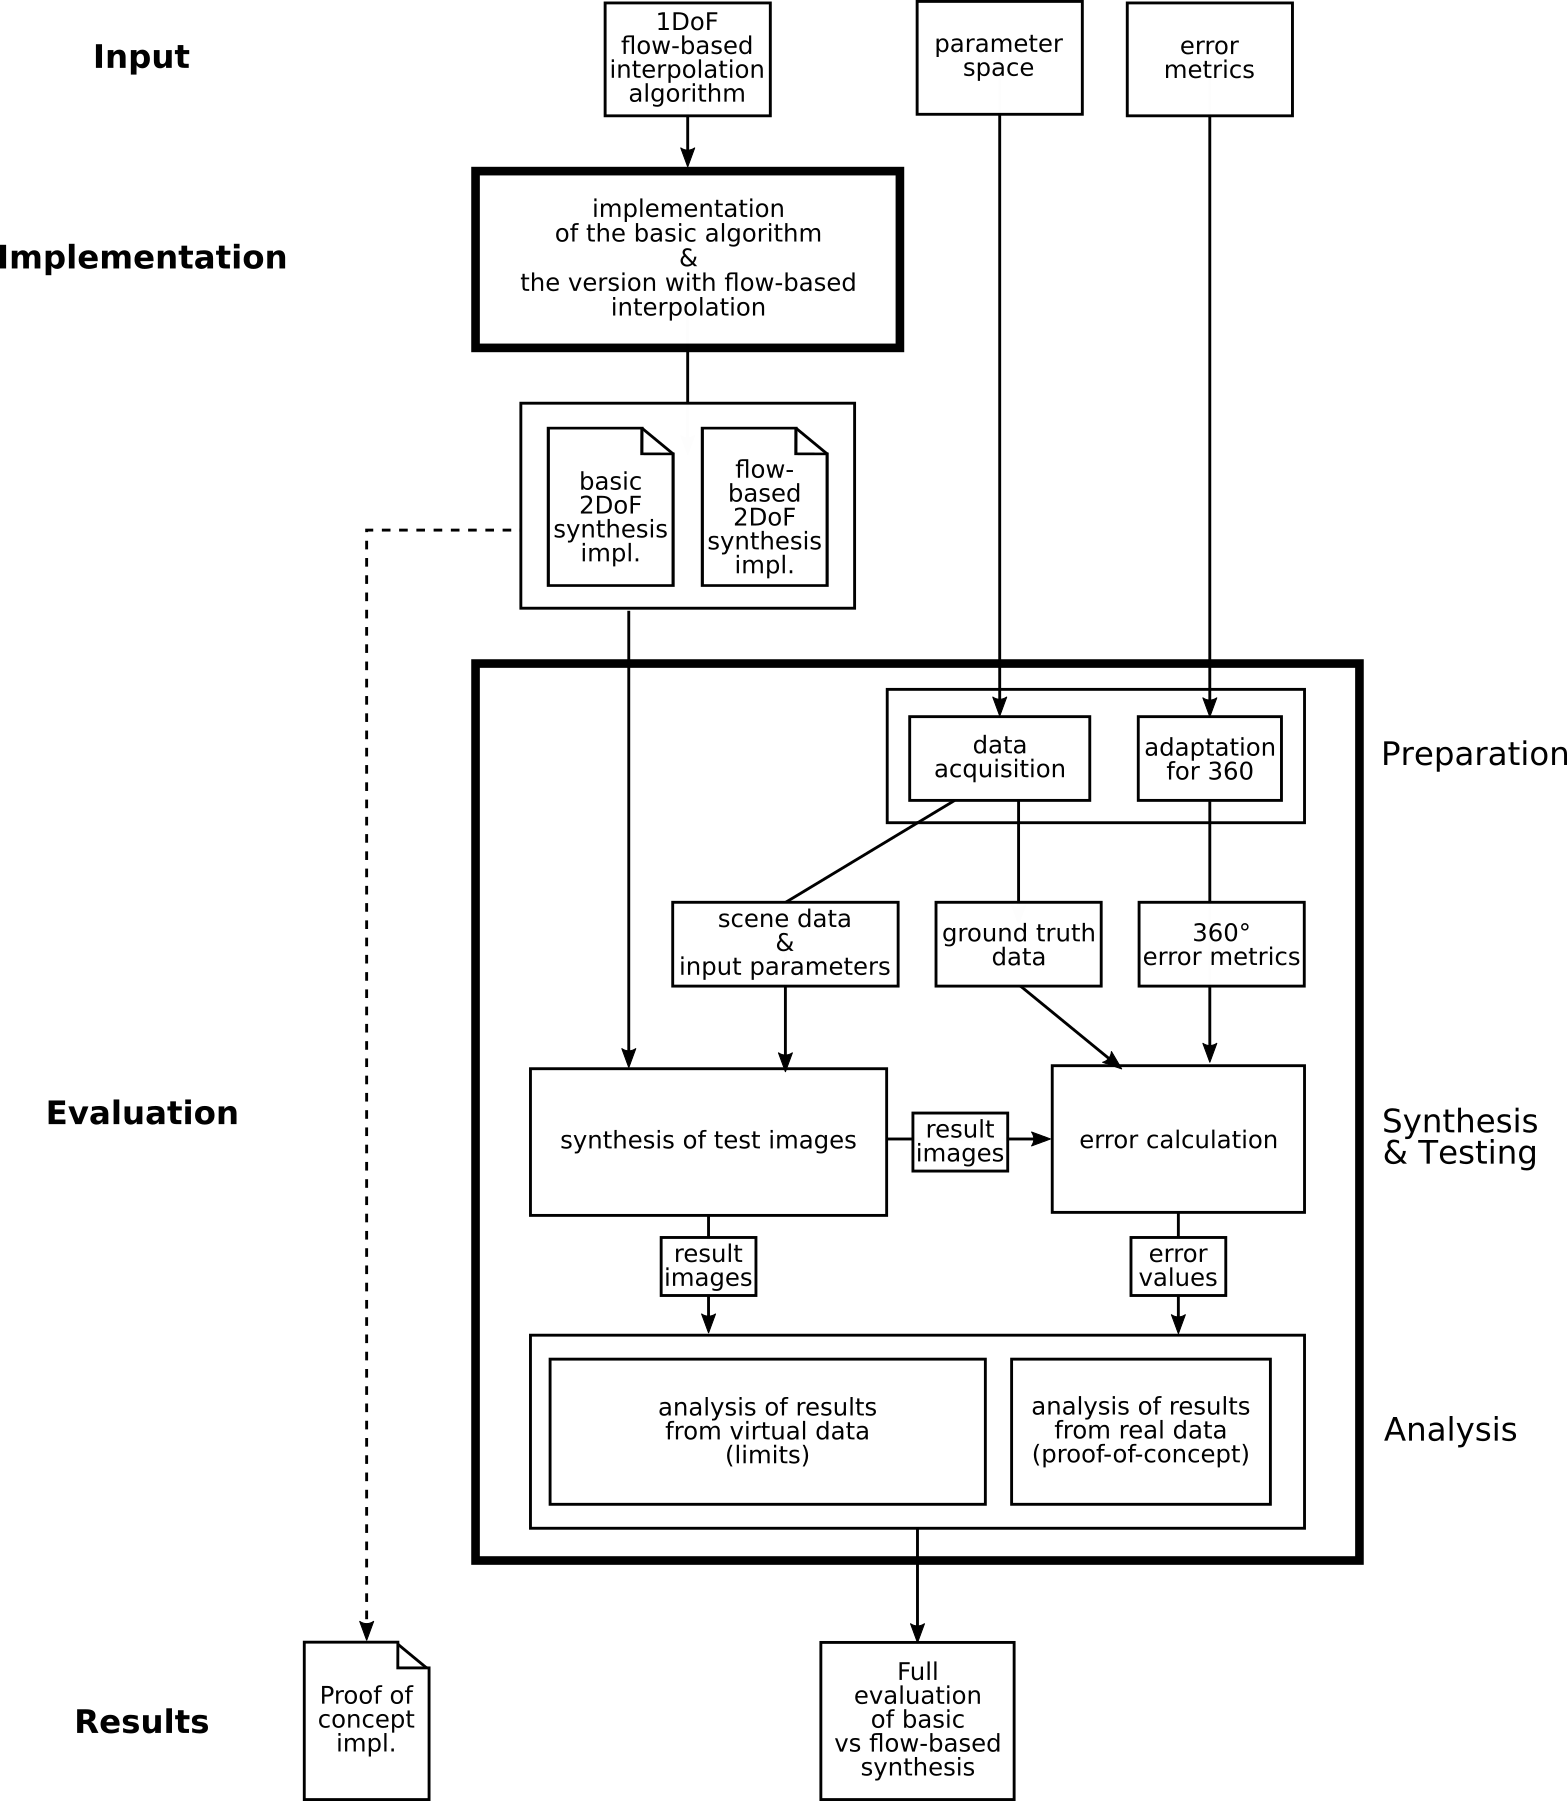
\includegraphics[width=0.9\textwidth]{01/methodology.png}
		\caption{Methodology}
		\label{fig:methodology}
\end{figure}

\section*{Results}
The results of this thesis are:
\begin{itemize}
  \item A basic proof-of-concept implementation of a 2DoF pixel-based synthesis algorithm with flow-based interpolation
  \item An evaluation of the results of this algorithm with a comparison of the pixel-based algorithm by itself versus with flow-based interpolation, proving that flow-based interpolation does improve the results of the basic algorithm in the majority of the examined cases
%  \item evaluation methodology for 360\degree images, including models and samples that can be used for benchmarking other methods \ar is it better than a naive algorithm?
\end{itemize}

The results of this thesis can be the basis of various future work. Since the implementation is a first attempt at combining the two methods, the problems and limitations discovered in the evaluation can be used to improve future versions. 

For example, the range of application can be extended to outdoor scenes, or to scenes with higher variation in distances to the camera. In these cases, the result implementation can be used as a base and the the problems and limitations found in the evaluation can be utilized as guidelines. Furthermore, it could be valuable to explore the possibility of combining this image-based rendering approach with approaches that use 3D geometry.
results
%- proof of concept implementation
%- evaluation of flow-based vs regular with several select parameters
%- yes, in the majority of evaluated cases, flow-based blending brings an improvement (given the optical flow algorithm produces accurate results)
%- but also has several major drawbacks that need to be handled

%national park:
%https://www.oculus.com/experiences/go/1524331530931445/?ranking_trace=0_1524331530931445_SKYLINEWEB_D8RtWgI7mmWKB0QLB
%mecca
%https://www.oculus.com/experiences/go/1125286047502859/?ranking_trace=0_1125286047502859_SKYLINEWEB_1QYbs8B1KfddDpRhA

%Along with this development, 360\degree cameras (i.e. cameras that capture the complete surroundings) have become more consumer-friendly and affordable as well. Previously, capturing a true 360\degree image was a fairly laborious. Several regular images that had been captured meticulously with a single camera facing in different directions, or a state-of-the art camera with several lenses, had to be stitched together in software. However, recently, development of designated 360\degree cameras with several built-in lenses and integrated stitching, has led to an increase in popularity with consumers\footnote{The price of a consumer-quality 360\degree camera is between approximately 200 and 1000 USD as of January 2021 (\url{https://www.techradar.com/news/best-360-degree-camera}, \emph{accessed 13/1/21}}.

%Given these developments, it stands to reason that using 360\degree cameras to create immersive viewing experiences for VR is a next logical step. In fact,
